\chapter{Tu primer vuelo, paso a paso}
\label{cap:primer-vuelo}

\begin{enpocas}
Un recorrido guiado: despegar y mantener el dron en el aire, mirar qué pasa por dentro, hacer una
órbita con viento y medirla, lanzar la búsqueda autónoma del incendio y, al final, volar con ArduPilot
y darle órdenes desde MAVProxy. Supone que la instalación (capítulo~\ref{cap:instalacion}) ya está hecha.
\end{enpocas}

\section{Paso 0: preparar la terminal}

Abre una terminal y escribe:
\begin{lstlisting}[style=bash]
source /opt/ros/jazzy/setup.bash
source ~/ros2_ws/install/setup.bash
\end{lstlisting}
Hazlo en \emph{cada} terminal nueva (o agrégalo a \cod{~/.bashrc}).

\section{Paso 1: despegar}

\begin{lstlisting}[style=bash]
ros2 launch cuadrirotor_sim simulacion.launch.py vehiculo:=tarot650 mundo:=bosque_grande controlador:=sta mision:=hover
\end{lstlisting}

Se abre Gazebo. El Tarot aparece sobre la base, despega suavemente y se queda a 3~m. A los 12 segundos
la cámara de la ventana empieza a seguirlo. En la terminal verás mensajes de los nodos.

\begin{figure}[H]
\centering
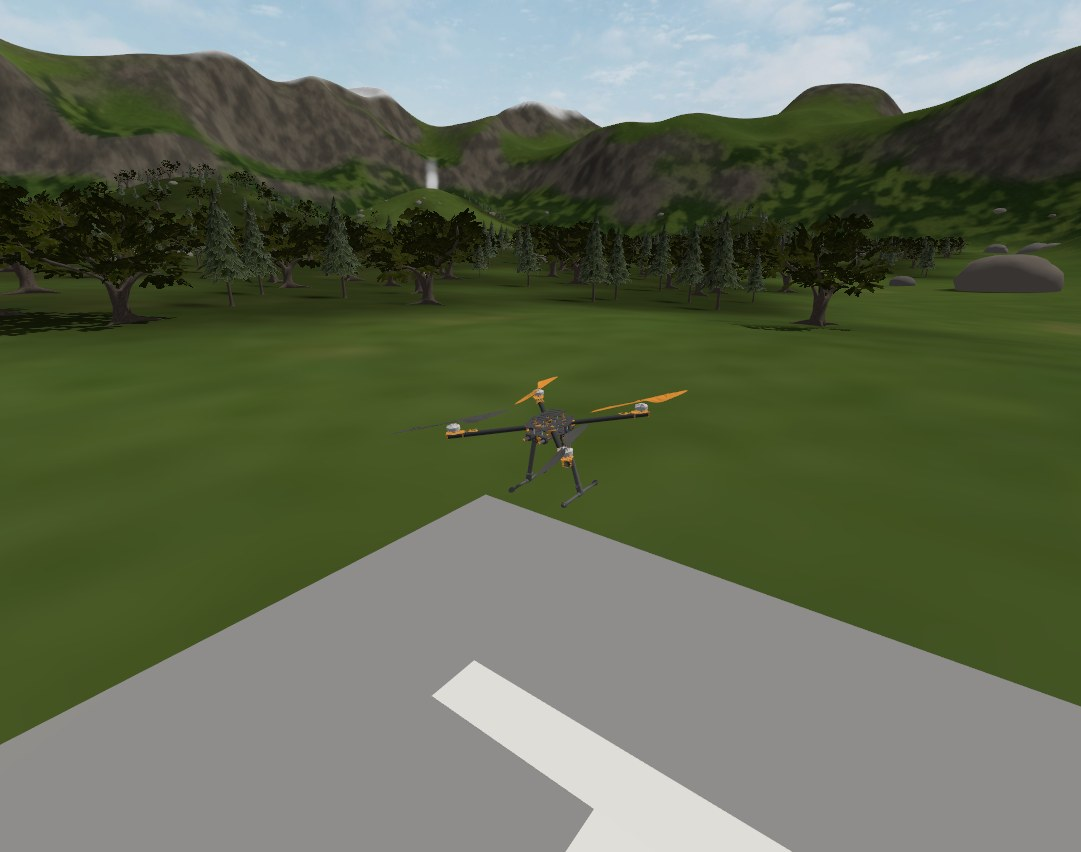
\includegraphics[width=0.75\textwidth]{gz_tarot_cerca.jpg}
\caption{Lo que debes ver: el Tarot en vuelo estacionario sobre la base.}
\end{figure}

\begin{consejo}
En Gazebo: rueda del ratón = acercar; botón izquierdo arrastrando = girar la vista; botón derecho
(o Shift + izquierdo) = desplazar. El botón ``play/pausa'' de abajo a la izquierda congela la física.
\end{consejo}

\section{Paso 2: mirar por dentro}

Abre una segunda terminal (con el Paso~0) y explora:
\begin{lstlisting}[style=bash]
ros2 node list                                                 # ¿quién está corriendo?
ros2 topic list                                                # ¿qué datos circulan?
ros2 topic echo /cuadrirotor/odometria --field pose.pose.position   # la posición del dron
ros2 topic echo /cuadrirotor/error                             # el error de seguimiento
ros2 run rqt_image_view rqt_image_view /cuadrirotor/camara     # lo que ve la cámara
\end{lstlisting}

\begin{figure}[H]
\centering
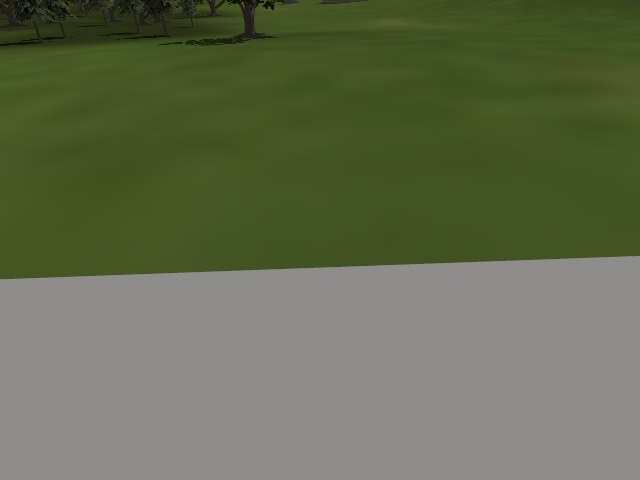
\includegraphics[width=0.6\textwidth]{gz_camara_dron.jpg}
\caption{La imagen de la cámara del dron sobre la base: el borde de la losa y el pasto.}
\end{figure}

Para cerrar la simulación, regresa a la primera terminal y presiona \textbf{Ctrl+C}.

\section{Paso 3: una órbita con viento, y medirla}

\begin{lstlisting}[style=bash]
ros2 launch cuadrirotor_sim simulacion.launch.py vehiculo:=tarot650 mundo:=bosque \
    controlador:=sta esquema:=implicito mision:=orbita viento:=true csv:=$HOME/mi_orbita.csv
\end{lstlisting}

El dron despega, va junto al foco del incendio y le da vueltas a 4~m de radio mirándolo; a los 15~s
empieza a soplar viento. Déjalo un par de minutos, ciérralo con Ctrl+C y mide:
\begin{lstlisting}[style=bash]
python3 ~/ros2_ws/src/cuadrirotor_sim/scripts/metricas.py ~/mi_orbita.csv
\end{lstlisting}
Verás el error RMS sin viento y con viento (unos 3 y 5~cm con el STA). Repite con
\cod{controlador:=pd} y compara: es el experimento central del proyecto.

\begin{ejercicio}
Abre \cod{~/mi_orbita.csv} en una hoja de cálculo o con Python y grafica \cod{x} contra \cod{y}: verás
el círculo de la órbita. Las columnas \cod{sx}, \cod{sy}, \cod{sz} son la variable deslizante y
\cod{k1x}, \cod{k1y}, \cod{k1z}, la ganancia adaptativa.
\end{ejercicio}

\section{Paso 4: la búsqueda autónoma del incendio}

\begin{lstlisting}[style=bash]
ros2 launch cuadrirotor_sim simulacion.launch.py vehiculo:=tarot650 mundo:=bosque_grande \
    controlador:=sta mision:=busqueda
\end{lstlisting}

Ahora el dron va solo:
\begin{enumerate}
  \item despega a 30~m sobre el suelo;
  \item recorre el bosque en serpentina (en la terminal: \emph{[patrulla] Recorriendo el bosque});
  \item cuando YOLO ve humo, se dirige hacia él (\emph{[hacia\_humo]});
  \item estima dónde está el foco y se acerca (\emph{[aproximacion]});
  \item al confirmarlo con las llamas, baja y empieza a orbitar, y escribe el aviso:
\end{enumerate}
\begin{lstlisting}
INCENDIO CONFIRMADO 2026-10-23 04:26:47
  GPS: 19.294219, -99.310000  (19°17'39.2"N 99°18'36.0"W)
  Mapa: https://www.google.com/maps?q=19.294219,-99.310000
\end{lstlisting}
Tarda entre uno y tres minutos según dónde esté el fuego. En la ventana de Gazebo, el panel
``Detección YOLO'' muestra lo que ve la red neuronal.

\begin{figure}[H]
\centering
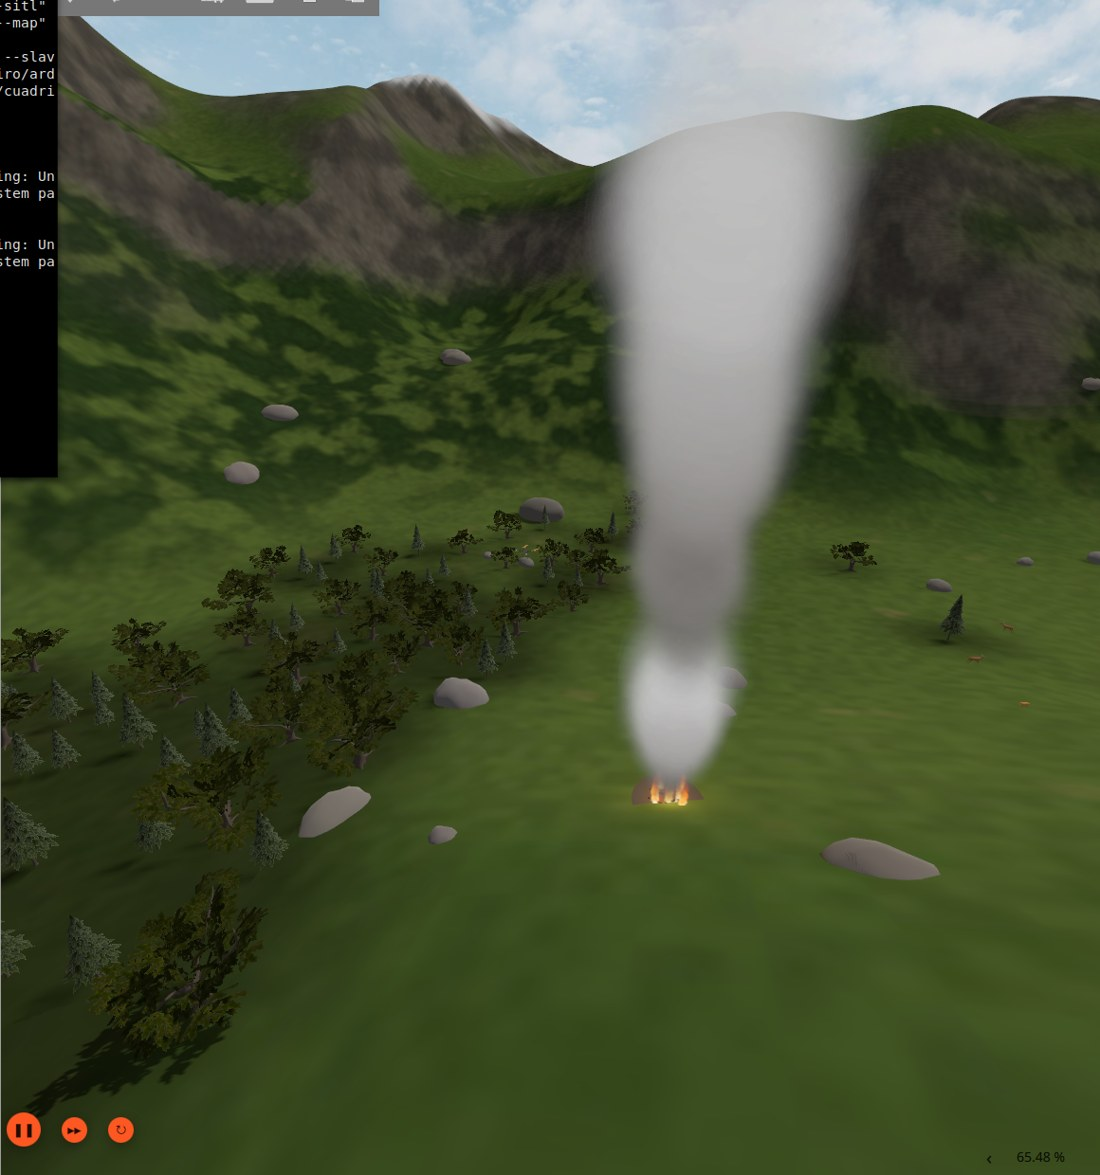
\includegraphics[width=0.6\textwidth]{gazebo_humo.jpg}
\caption{El dron llegando al incendio.}
\end{figure}

\begin{ejercicio}
Pon el incendio en otro lugar y observa cuánto tarda en encontrarlo:
\begin{lstlisting}[style=bash]
ros2 launch cuadrirotor_sim simulacion.launch.py vehiculo:=tarot650 mundo:=bosque_grande \
    controlador:=sta mision:=busqueda foco_x:=-150 foco_y:=60
\end{lstlisting}
Desde otra terminal: \cod{ros2 topic echo /cuadrirotor/busqueda/cobertura} muestra qué porcentaje del
bosque ya vio.
\end{ejercicio}

\section{Paso 5: volar con ArduPilot y darle órdenes}

\begin{lstlisting}[style=bash]
ros2 launch cuadrirotor_sim simulacion.launch.py vehiculo:=tarot650 mundo:=bosque_grande \
    controlador:=ardupilot mision:=busqueda
\end{lstlisting}

Se abren cinco ventanas acomodadas solas: arriba a la izquierda la terminal \textbf{MAVProxy}, debajo
la consola y la terminal de ArduCopter, Gazebo al centro y el mapa a la derecha. Tras $\approx$30~s de
revisiones, ArduPilot arma, despega y sigue la misma búsqueda. En el mapa verás la ruta planeada en
cian y lo recorrido en magenta.

\begin{figure}[H]
\centering
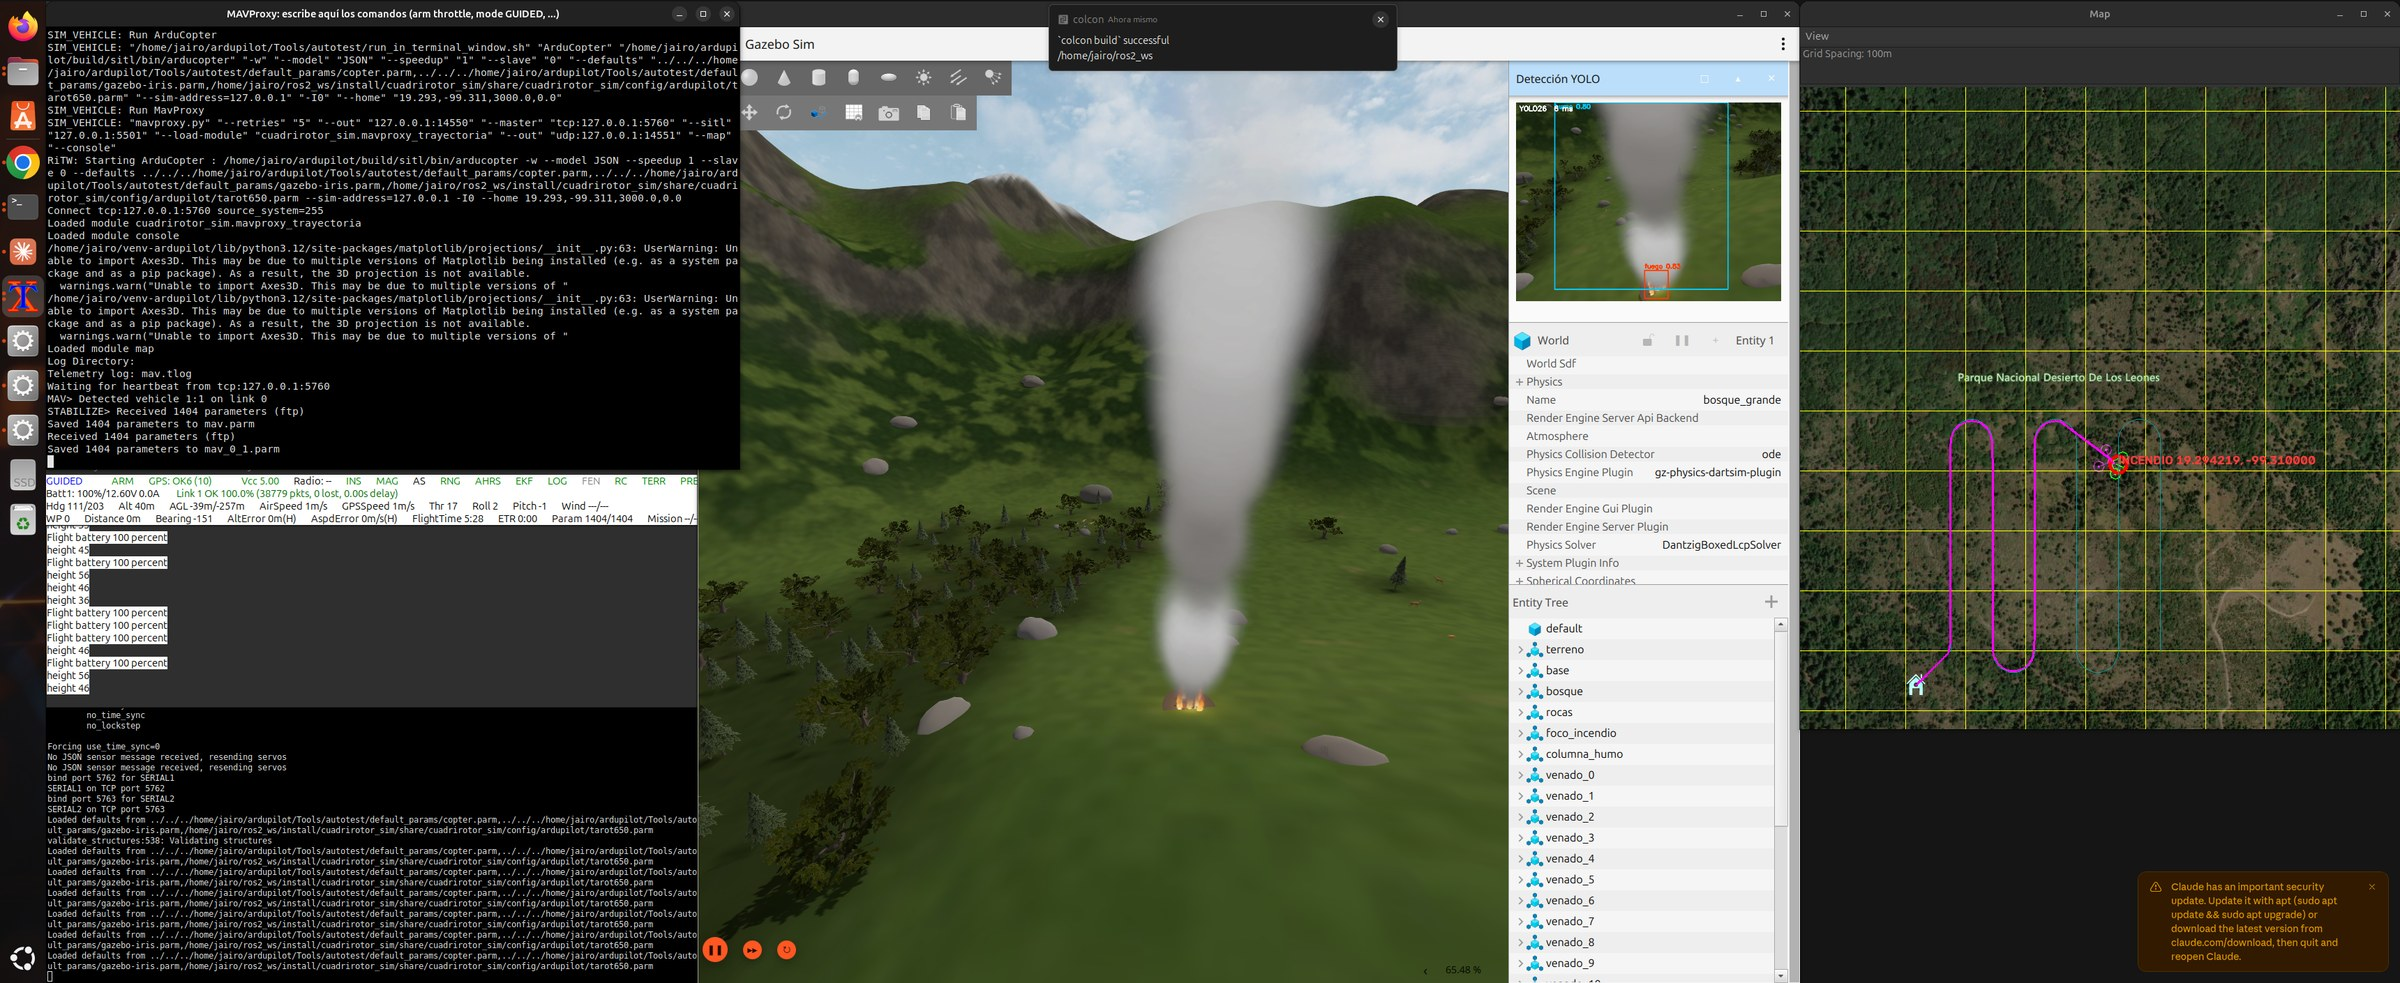
\includegraphics[width=\textwidth]{sitl_pantalla.jpg}
\caption{La pantalla con ArduPilot al confirmarse el incendio.}
\end{figure}

Escribe en la terminal MAVProxy (donde dice \cod{MAV>} o \cod{GUIDED>}):
\begin{lstlisting}
mode LOITER          # el dron se detiene donde está
mode GUIDED          # retoma la búsqueda
mode RTL             # regresa a la base y aterriza
trayectoria borrar   # limpia la línea magenta del mapa
\end{lstlisting}

\begin{aviso}
Si tomas el control con un modo distinto de GUIDED, la misión no puede mover al dron hasta que
regreses a \cod{mode GUIDED}. Y si aterriza con RTL y se desarma, hay que reiniciar la simulación.
\end{aviso}

\section{Qué hacer si algo falla}

\begin{longtable}{>{\raggedright\arraybackslash}p{5.5cm}p{9.5cm}}
\toprule
\textbf{Síntoma} & \textbf{Qué revisar} \\ \midrule \endhead
\emph{Package 'cuadrirotor\_sim' not found} & Falta \cod{source ~/ros2_ws/install/setup.bash} en esa terminal. \\
Gazebo abre pero el dron no aparece & Mira la terminal: un error en rojo del \emph{launch} dice qué falló. \\
La simulación va muy lenta & Cierra otros programas; prueba \cod{gui:=false}. Revisa el factor de tiempo real abajo a la derecha de Gazebo. \\
YOLO no detecta nada & ¿Existe \cod{~/.venvs/yolo}? ¿Tiene GPU? Mira los mensajes de \cod{detector_yolo}. \\
Quedan procesos de una simulación anterior & Ciérrala con Ctrl+C y espera unos segundos; si algo queda, búscalo con \cod{ps aux | grep gz} y termínalo por su número (PID). \\
ArduPilot no arma & Espera: el EKF tarda $\approx$30~s. La consola de MAVProxy dice qué revisión falla. \\
\bottomrule
\end{longtable}
